\section{Experiments}
\dmcmt{Measure time taken by refinement?}
\todo{Talk about numpy for matrix ops and scipy for hcluster}

We have implemented our method in python, using a linkage-matrix\todo{cite,
maybe from the scipy docs} based
data structure to store the tree, and have precomputed and cached several
operations that may need to be repeated every refinement iteration. This allows
us to quickly perform the merge and split operations and calculate the
scores, \dmcmt{TODO ref earlier sections} without having to do (relatively)
expensive tree traversal operations in each iteration of the abstraction
refinement loop. 

Using this implementation, we have performed three sets of experiments to
demonstrate the usefulness of our technique. We first use our abstractions to
attempt to verify safety properties of the \acasxu networks. However,
abstractions may be useful in other
domains as well, \dmcmt{What? Any formal analysis beyond verification, for
example, formal explainability \todo{cite gk} scalability is sensitive to size.
So abstractions can give smaller nets with some guarantees. Check Jan Kretinsky,
guarantees not enough, cite. Motivate section 4.3}, in particular to obtain compressed networks with certain safety guarantees behind them. To
demonstrate this, we use our implementation to compress networks trained on the
MNIST networks in the second and third set of experiments. \dmcmt{This needs to
intro our story better}

\dmcmt{TODO add gh link and exp machine details}

\subsection{\acasxu}
\dmcmt{These set of experiments still needs to be rerun}

In these set of experiments, we have taken the \acasxu set of
networks \todo{add detailed table} and
properties and attempt to verify them using a \cegar approach. We use our
technique to generate the abstraction, and attempt to verify the property on the
abstract network using an existing neural network verification solver. If the
solver returns a counterexample, and if that counterexample is not spurious, we
use that counterexample as a reference point for score calculation \todo{Ref
prev sec} to select the culprit neuron. \todo{Ref prev section, maybe already
there, remove} With the culprit
neuron selected, we then refine the network.

\begin{table}
\begin{tabular}{ |c|c|c|c| }
\hline
Benchmarks &    \% Verified &  Avg Reduction &  Avg Time \\
\hline
safe       &        40.404  &         4.4875 &   14.198  \\
unsafe     &       100      &        55.6071 &   12.7916 \\
\hline
\end{tabular}
\caption{Summary of \acasxu Results\todo{Fix formatting}}
\label{t:acas-summary}
\end{table}

The results are summarised in table \ref{t:acas-summary}. The solver we used was
\abcrown. \dmcmt{Note, avg time and network size here doesn't include
timeouts. Also, for reduction rate, the original network size is taken to be
600, since the re-merging optimization is not there in this data. With that
optimization added, we should compare against 300. Also, the full verification
rate is 100\% because its not a full set of experiments, this will potentially
be a lot lower.} 

We notice that for the unsafe cases, we are able to refute the
properties via a counterexample obtained on a significantly smaller network.
\dmcmt{But what about the safe cases, what do we say?}. In fact, for most
networks, we are able to refute based on a counterexample from the fully
abstracted network of size $18$. \dmcmt{This is not there in this small summary
table, but is clear from the full data table. Maybe link to that somewhere
in the appendix?} Note that since we use only two classes in our
fully abstracted network as opposed to 4 in \cite{cegar-nn}, the size of this
network is significantly smaller. In other networks, we are are able to get a
counterexample on a network with size very close to the original network.

For the safe cases, we see that the size of the abstracted networks are large
for instances that did not time out.  This is in line with what was observed in
\cite{cegar-nn} \dmcmt{Can we claim this? It's not immediately clear from their
paper, maybe we need to show our recreation of their experiments? Also, this
split is not clear from the table}. For other instances, the timeout happened
due to the solver timing out on the abstract query. \dmcmt{While the sizes of
the networks on which this to happened are small, does that not say
something negative about our abstraction?}

\begin{figure}
    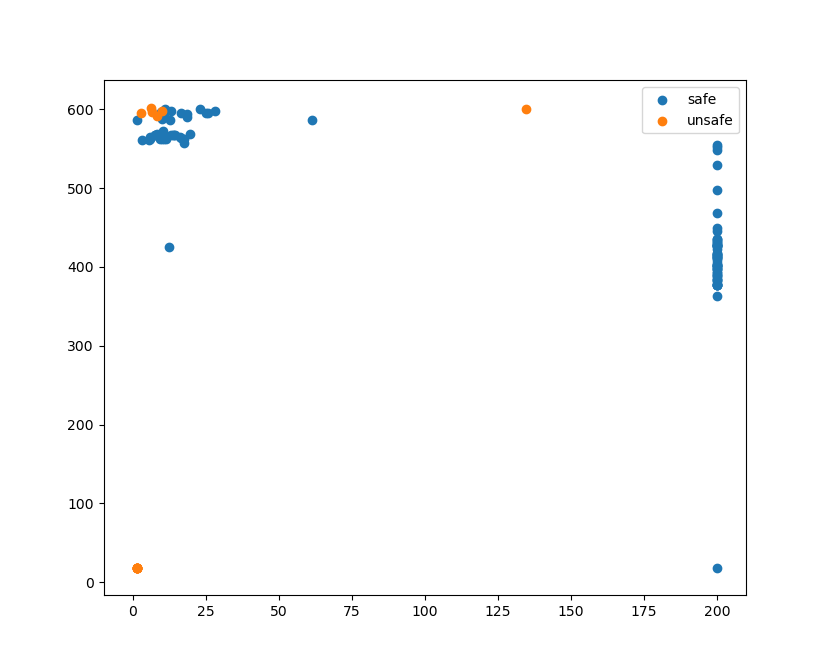
\includegraphics[scale=0.4]{figs/acas-scatter.png}
   \caption{Scatter plot of abstract network sizes vs time in seconds for
   \acasxu}
   \label{f:acas-scatter}
\end{figure}

Figure \ref{f:acas-scatter} shows the network sizes and times of the \acasxu
networks as a scatter plot. \dmcmt{This includes to and non-to}. Note that the
time taken here is dominated by the solver call time \dmcmt{Should we measure
and report this precisely?} We see that the time taken by the solver call on
these networks is not at all correlated with the network sizes. For instances,
for the safe cases, there are several networks of sizes ranging from $350$ to
$600$ \relu nodes all of which time out on the solver call. Similarly, for the
unsafe networks, several $600$ size networks take less than $25$ seconds. In
fact, we found that the time taken by the solver call on a particular network is
more dependent on the solver (and configuration of the solver) used than on the
size of the network. Due to this, in the following experiments, we measure the
accuracy of the networks obtained via abstraction instead of making solver calls
to determine the effectiveness of the abstraction. \dmcmt{Is this okay? Can it
be instead argued that the variance is due to the networks themselves, so the
abstraction is not necessarily useful?
Maybe trying with other configs and showing the variance?}

\subsection{Robustness on \mnist}
\dmcmt{What about doing these experiments on ACAS?}
\dmcmt{Do pgd then samples}

In this section, we start with our abstraction and progressively refine it using
our refinement technique, measuring the number of spurious counterexamples at
each step. To perform the refinement at each step, we try four methods to
perform the culprit neuron selection. The first method 'random' simply chooses a
culprit at random, and serves as a baseline. For the other three methods, we
choose a number of reference points to calculate scores, and choose the culprit
neuron with the highest score. For 'samples', the reference points are random
generated input points that satisfy the precondition. For 'pgd', the samples are
generated via a PGD \todo{cite} attack on the abstract network at each step. For
'samples-pgd', we do some initial refinement steps using the randomly generated
samples, when all the samples have been exhausted, we then perform 'pgd'. We use
the implementation of 'pgd' inside \abcrown for our experiments.

\begin{figure}
    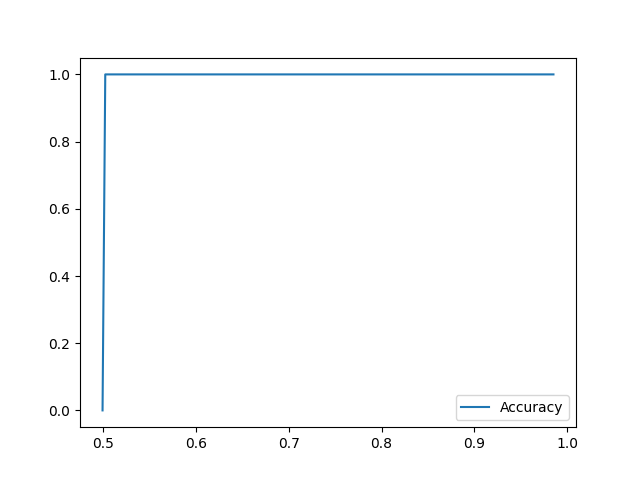
\includegraphics[scale=0.4]{figs/mnist_2_256_prop_0_0.03_samples.png}
    \caption{Accuracy vs Reduction Rate plot for \mnist of size $2 \times 256$
        with $\epsilon$-Robustness property. Refinement done via the 'samples'
    method.}
    \label{f:mnist-prop-samples}
\end{figure}
\begin{figure}
    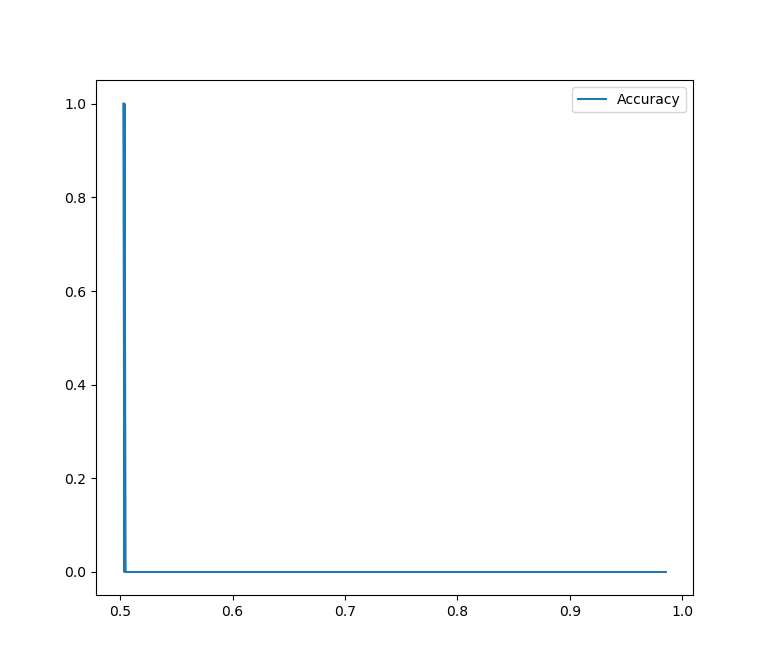
\includegraphics[scale=0.4]{figs/mnist_2_256_prop_0_0.03_pgd.png}
    \caption{Accuracy vs Reduction Rate plot for \mnist of size $2 \times 256$
        with $\epsilon$-Robustness property. Refinement done via the 'pgd'
    method.}
    \label{f:mnist-prop-pgd}
\end{figure}

Figure \ref{f:mnist-prop-samples} \ref{f:mnist-prop-pgd} shows a typical plot
for these experiments.  Here accuracy measures the number of true
counterexamples within a random sample
drawn from a region satisfying the pre-condition. \dmcmt{Should I plot and talk
in terms or spurious counterexample rate instead?} We see that as we refine the
network and the reduction rate reduces (moving right to left along the graph),
the accuracy remains close to zero. At some point however, the accuracy jumps up
sharply and becomes close to $100\%$. This indicates that there are a few
critical refinement steps that remove almost all spurious counterexamples. This
may be due the fact that with epsilon robustness properties that are being
explored here, the pre-condition region may be very small, so a single
refinement step may change the behavior of the network on that small region in a
way that eliminates all possible spurious counterexamples from that region.
\dmcmt{Is this expl okay?}
\dmcmt{BaB and abstract interp based methods like \abcrown are successful on
such props because of this, discuss this?} \dmcmt{Also, other graphs are
present. For eg, some random sampling graphs show peaks in the middle
(2..random), and some pgd graphs are flat lines (4,6..pgd). Discuss
these?}

\begin{table}
\begin{tabular}{|c|c|c|c|c|}
    \hline
    Net Size     & Cex Method  & Reduction & Accuracy & No. Steps \\
    \hline
    $2\times256$ & random      & $49.1\%$  & $100\%$  & $ 809$    \\
    $4\times256$ & random      & $49.6\%$  & $100\%$  & $1778$    \\
    $6\times256$ & random      & $49.7\%$  & $100\%$  & $2602$    \\
    $2\times256$ & samples     & $50.3\%$  & $100\%$  & $  27$    \\
    $4\times256$ & samples     & $49.9\%$  & $100\%$  & $ 648$    \\
    $6\times256$ & samples     & $47.9\%$  & $100\%$  & $1199$    \\
    $2\times256$ & pgd         & $50.4\%$  & $100\%$  & $  28$    \\
    $4\times256$ & pgd         & $88.6\%$  & $  0\%$  & $  14$    \\
    $6\times256$ & pgd         & $83.3\%$  & $  0\%$  & $  82$    \\
    $2\times256$ & samples-pgd & $50.3\%$  & $100\%$  & $  27$    \\
    $4\times256$ & samples-pgd & $49.9\%$  & $100\%$  & $ 648$    \\
    $6\times256$ & samples-pgd & $47.9\%$  & $100\%$  & $1209$    \\
    \hline
\end{tabular}
\caption{Summary of \mnist Results on a single robustness property \todo{Fix
formatting} \dmcmt{Include Times?}}
\label{t:mnist-prop-summary}
\end{table}

Table \ref{t:mnist-prop-summary} summarizes these results for multiple \mnist
networks and multiple refinement methods. Accuracy here refers to the final
accuracy of the best network found when the refinement process stops due to lack
of counterexamples. Firstly, we find that 'pgd' performs poorly on the $4$ and
$6$ layer networks, where while the number of steps are relatively low and the
reduction rate is high, the accuracy is very low. This is because the \abcrown
implementation of \pgd fails to find a spurious counterexample early on in the
refinement process for these instances, leading to early termination without
ever hitting the accuracy jump. 

Apart from these exceptions, the other instances and methods seem to perform
comparably on the same network in terms of reduction rate. This is evidence for
the fact that, within the limited search space of abstractions defined by our
tree, there exists a strong enough abstract network with a good reduction rate,
and that it is possible to find this network via a \cegar-like approach. 

Further, we see significant difference in the number of steps taken by 'random'
and the other methods in finding the abstract network. This indicates that our
heuristics for finding a culprit neuron to base the refinement on indeed
shortens the search for the refined network. We also observe that
'samples','samples-pgd' and for the $2$ layer network 'pgd' take similar number
of refinement steps, indicating that each method may be taking close to the
optimal set of refinement steps. So, although the 'pgd' method
incurs a significant time overhead \dmcmt{Measure?} it does not necessarily
provide any benefits.\dmcmt{Last two paragraphs okay? Refer to this
in intro of experiments section? Also, pgd does not produce improvement (unlike
in cleverest). This is prob because global view, and cegarette is about doing an
eager attack before solver call. Discuss this? So two potential angles on this,
what Ive written vs global view angle.} 

\subsection{Compression with Guarantees on Critical Classes}

In several safety-critical applications of \dnn as classifiers, there are
certain `critical` classes for which a false negative classification is far more
dangerous than a false positive one. For example, for medical diagnosis and
collision detection, a false negative is far more dangerous than a false
positive.

Safety critical analysis of neural networks is highly sensitive to the size of
the network. While several neural network compression techniques exist
\todo{cite}, they provide limited formal guarantees \dmcmt{ Talk about Jan? How?
} connecting the behavior
of the compressed network and the original network. Thus, any analysis,
including, for example, formal explainability or verification, done on the
compressed network cannot easily be lifted to the original network. This lack of
guarantees also limits the usefulness of these compression techniques as
optimisation steps when deploying a network to a resource-constrained
environment. 

Our theoretical framework for abstraction allows us to produce compressed
networks with the formal guarantee that the abstraction process will not
introduce any new false negative. We do this by marking the output neuron $n_c$
corresponding to the critical class in the output layer as inc, and all other
neurons in that layer as dec.  Then, for any input that the concrete network
classified into the critical class, $n_c$ will have the largest value in the
output layer, and as it has been marked as inc, it will continue to have the
larges value in the output layer for the abstract network as well. Thus, the
abstract network will also classify this input as critical. We will however pay
for this compression by introducing false negatives, as we will demonstrate
shortly. \dmcmt{Last sentence okay?}

\begin{figure}
    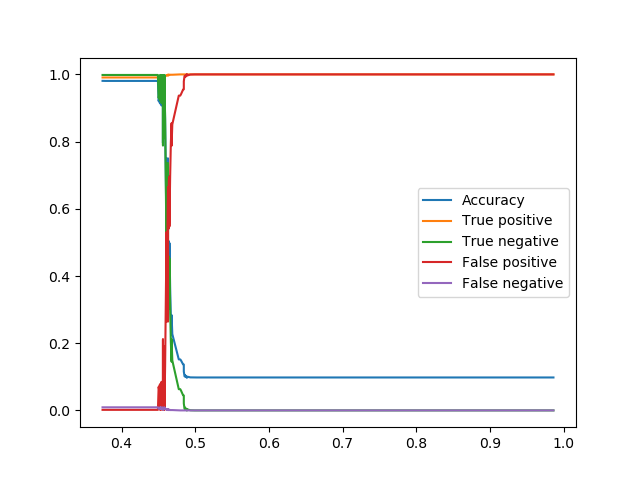
\includegraphics[scale=0.6]{figs/mnist_2_256_class_samples.png}
    \caption{Accuracy and True/False Positive/Negative Rates vs Reduction Rate
        plot for \mnist of size $2 \times 256$ with critical class 0. Refinement
        done via the 'samples' method.}
    \label{f:mnist-class-samples}
\end{figure}

We demonstrate the effectiveness of our abstraction method as such a compression
with guarantees technique via some experiments on \mnist and show the results in
figure \ref{f:mnist-class-samples}. We set the class '0'
as the critical class, and use our abstraction technique to obtain a compressed
network. Then, we use the 'samples' method described previously to progressively
refine the network (moving right to left) , plotting the accuracy, false/true
positive/negative rates as we go along. For this plot, the samples were drawn
from the \mnist training dataset, and the accuracies were plotted using the
\mnist test dataset.

We notice that, as guaranteed by the theory, the false negative rate never
increases, even as the reduction rate approaches close to $100\%$. Thus, even
for highly compressed networks, we never introduce any new false positives, and
in fact, the false negative rate improves, as some of the points that are going
to be newly classified as positive may in fact be true positives. However, as
discussed before, we do pay for the compression by introducing false positives,
which rises steeply in the graph. This is again similar to the behavior seen in
the previous section, where a few refinement steps leads to the elimination of
most of the spurious counterexamples all at once \dmcmt{The reason may not be
the same} 

We note that from the graph, even at around $45\%$ compression rate,
we find that the false positive rate is close to that of the original network.
This shows that our abstraction technique can find effective compressions with
the guarantee that no false negatives have been introduced.
